\documentclass[conference]{IEEEtran}
\usepackage[utf8]{inputenc}
\usepackage{ifpdf}
\renewcommand{\sfdefault}{cmss}
\renewcommand{\rmdefault}{cmr}
\renewcommand{\ttdefault}{cmtt}
\usepackage[english]{babel}
\usepackage[pdftex]{graphicx}
\usepackage{caption}
\usepackage{float}
\usepackage[colorlinks,filecolor=blue,citecolor=green,unicode,pdftex]{hyperref}
\usepackage{cmap}
\usepackage{amsmath,amssymb}
\usepackage[mathcal]{euscript}
\hypersetup{colorlinks=true, linkcolor=blue, citecolor=blue, filecolor=blue, urlcolor=blue, pdftitle=1, pdfauthor=, pdfsubject=, pdfkeywords=}

\sloppy
\clubpenalty=0
\widowpenalty=0
\raggedbottom

\begin{document}

\title{Technology for application family creation based on domain analysis}

\author{
	\IEEEauthorblockN{Gudoshnikova Anna}
	\IEEEauthorblockA{
		Chair of informatics \\
		St.-Petersburg State University \\
		St.Petersburg, Russia \\
		Email: gudoshnikova.anna@gmail.com
	}
\and
	\IEEEauthorblockN{Yurii Litvinov}
	\IEEEauthorblockA{
    	Software Engineering chair \\
    	St.-Petersburg State University \\
    	St.Petersburg, Russia \\
    	Email: y.litvinov@spbu.ru 
	}
}

\maketitle

\begin{abstract}
The theme of code reuse in software development is still important. Sometimes it is hard to find out what exactly we need to reuse in isolation of context. However, there is an opportunity to narrow the context problem, if applications in one given domain are considered. Hence, the problem of domain analysis arises. On the other hand, there is metaCASE-techonology that allows to generate code of an application using diagrams. The main objective of this article is to present the technology for application family creation which connects the metaCASE-techonology and domain analysis. We propose to use feature diagrams to describe variability in a domain and then create domain-specific visual language that allows to connect and configure existing feature implementations thus producing an application. This technology supposed to be especially useful for software product lines.
\end{abstract}

\begin{IEEEkeywords} domain analysis; metaCASE-technology; domain-specific language; application family \end{IEEEkeywords}

\section{Introduction}
The term ``reuse'' in software engineering is closely associated with context. Reuse objects can be programs, parts of programs, specifications, requirements, architectures, test plans, etc. Reuse of one object leads to reuse of another object. This means, there is a need to reuse something more than just code, i.e. there is a call for increasing the abstraction level. It is commonly supposed that reuse, as some kind of activity, can be divided into groups according to what should be reused: components, process for gaining the product, technology or knowledge. At all accounts any reuse object cannot be discussed without environment, where the given object exists. Hence, the context problem still remains. 

However, if we reuse objects in one domain, the context issue may be narrowed. The product line implies that there is a common part, it can be: (1) architecture, (2) components, (3) algorithms, (4) methods, etc. --- and this part exists in the same context. This fact facilitates the reuse problem. Consequently, the common part must be reused.

Gathering information about the domain is the crucial step in the whole process of software development. Nowadays applications in one domain are often designed independently; this approach leads to increase of development time and cost. Usually such applications have similar functionality, so the reuse problem moves to the forefront in an attempt to speed up the development and to decrease the cost for systems in one domain. The reuse process in one domain supposes the necessity of the domain analysis activity. At present domain analysis in software life cycle is performed in informal way. There are some domain analysis tools, but such tools are not integrated with development tools. As the result of the domain analysis activity some diagrams just are put up on the board, and do not take part in following process of software design. The risk of incorrect understanding of domain-dependent knowledge increases. Therefore, many peculiarities of the domain may be missed in development process because of the factor of human error. This fact may lead to development of the product which does not satisfy requirements at all. Hence, there emerged a need for a tool in which domain analysis activity would play a vital role in software development process, i.e. based on this activity would be possible to generate some design model, so developers and other process actors could rely on this model. At the present day there is no tool that could allow to solve this problem.   

One possible solution for this problem is the use of domain analysis tool in model-driven development, or, more precisely, domain-specific modelling. Domain-specific approach uses visual languages to specify system under development, but, contrary to general model-driven approach which uses general-purpose visual languages like UML, domain-specific languages are tailored specifically for given domain or a set of problems. Existing studies~\cite{tolvanen2016challenges,baker2005model,kieburtz1996software,kelly2000visual} show that due to closeness to a problem domain and the ability to generate complete application by visual models domain-specific languages boost development productivity by 3 to 10 times compared to general-purpose languages. It is clear that developing a tool for domain-specific language ``from scratch'' for each domain will be prohibitively costly, so special systems are used that allow to declaratively specify syntax of a language and to automatically generate such tools as visual editor, source code generators, constraints checkers and so on. Such systems are called DSM platforms, most known of these is MetaEdit+~\cite{tolvanen2007advanced,tolvanen2009metaedit,kelly2008domain}, Eclipse GMP~\cite{gronback2009eclipse,viyovic2014sirius}, Microsoft Modeling SDK~\cite{cook2007domain}.

Main idea of domain-specific modeling is to use a number of visual languages in one tool to develop a complete system. Every language can provide a different point of view on a system. We propose to exploit this idea to automatically produce useful artefacts from the results of domain analysis thus seamlessly integrating this phase into development process (such as~\cite{koznov2011process}). For that, we will use specific visual language to perform domain analysis and to build domain model, language simple enough to be useful to analysts and domain experts who do not necessarily possess programming skills. Then, using this domain model, we will generate actual domain-specific language that will allow to configure various existing pre-built components and integrate them to generate a working application. As we will see, this language will also typically be very simple so that non-programmers can use it. The only real coding in the proposed approach occurs when creating components from which applications will be built, but for product lines these components will already exist anyway, as they will in a case when a team develops many applications in one domain for some time. Not all steps in proposed approach are fully automatic, as a visual language needs tailoring after generation from domain model --- we still need to manually specify shapes of its elements (to be familiar for domain experts) and configure properties which depend on existing components and can not be derived from domain model. It is also possible that generated application will need tailoring by hand, but generation can significantly lower the effort needed to create application.

Main contribution of this research-in-progress paper is a novel approach to product line development and assets reuse. Also an implementation of technology which uses this approach is presented. Our technology is based on QReal DSM platform~\cite{kuzenkova2013qreal}, an open source tool developed by Software Engineering chair of St. Petersburg State University\footnote{GitHub repository and home page of QReal project, URL: https://github.com/qreal/qreal (03.04.2016)}. An evaluation of proposed approach is also presented, but on a rather simple problem, so a much wider evaluation is needed for this study to be considered complete, such as the applicability of this approach to complex real-life situations and determining actual productivity boost on real-life problems.

The rest of this paper is structured as follows: in section~\ref{chapter:approaches} most important terminology for domain analysis is given, also related works are considered. In section~\ref{chapter:proposed} we present our method and its implementation as development platform, in section~\ref{chapter:evaluation} an example of application of our approach is given, we will consider a family of Android gamepads for remote control of various robot models. Section~\ref{chapter:conclusion} concludes the paper.

\section{Domain analysis approaches}
\label{chapter:approaches}
There is no any clear and long-standing definition of the term ``domain analysis''. Almost all papers, in which this term is considered, go back to 80s-90s of the twentieth century. It was then that scientists, taking into account rapidly growing technologies, were thinking about global reuse. Always projects are developing for concrete user needs, so then the term ``domain'' took the definition. Domain is the field of expertise, problems in which the software intends to solve. According to Rugaber~\cite{rugaber1994domain}, the domain is described in terms of glossary, some assumptions, architecture approach and literature. 


Then the question arise, how we need to analyze the domain for acquiring the necessary information. At present, the information gathering into knowledge bases is understood under the term ``domain analysis''. Although, Prieto-Diaz~\cite{prieto1988domain} confirms that domain analysis is an activity, which is held before system analysis and its output is used for system analysis to the same degree as system analysis’s output is used for system design.  There are other definitions of the term ``domain analysis''. Ferre~\cite{ferre1999evaluation} has presented definitions, such as: (1) the process of identification, organization and presenting the relevant information of a given domain, (2) the process, in which the customer’s knowledge are identified, concretized and systemized. The relevant information of the domain should be presented in objective, readily available way, such way is called ``domain model''. Mernik~\cite{mernik2005} specifies that the domain model includes not only glossary, but also must describe commonalities and variabilities of terms. Such model should precisely set bounds of the domain, i.e. clear and exact characterize a range of questions, which are considered in the domain. Term variabilities allow to define exactly, what information must be specified in concrete system implementation. Term commonalities are used for defining a set of shared operations between different applications. Implementing commonalities and adding the gained model  with information, which can be specified in instance of the concrete system, a set of different systems can be obtained based on one common model. In such manner, based on one domain model, the set of different systems in given domain can be implemented. Taking into account definitions above mentioned, we can conclude that domain analysis is the activity of forward system analysis, which goal is to provide the domain model. 

As stated above, at present in many software companies the term ``domain analysis'' is understood as information gathering into some knowledge bases, but it is obvious that there are disadvantages of this approach. It may lead to incomplete glossary, absence of agreements about understanding some terms in the domain, so any misunderstanding of domain can result in an improper product. Therefore, several dozens of years ago were introduced some formal approaches for domain analysis. Here will be mentioned some of them. Main objective any domain analysis approach is to gain the domain model.  


Despite different understanding of the term ``domain analysis'', Arango~\cite{arango1994domain} showed that all formal domain analysis methods follow the general process for obtaining the domain model. This process includes next stages: (1) domain characterization, (2) data collection, (3) data analysis, (4) classification and finally (5) evaluation of domain model. There are following domain analysis approaches: 1) DARE (Domain Analysis and Reuse Environment)~\cite{frakes1998dare}. The crucial idea of this method is to create the domain book, that will include the universal architecture and library of reusable components. 2) DSSA (Domain-Specific Software Architectures)~\cite{taylor1995software}. Given approach allows to create a domain glossary with the aid of use case analysis. 3) ODE (Ontology-based Domain Engineering)~\cite{falbo2002ontological}. This approach connects the ontology idea with object-oriented approach. Ontology includes  terms and their connections, definitions, properties and constraints. Library of objects is built based on mapping ontology with object-oriented entities. 4) FODA (Feature-Oriented Domain Analysis)~\cite{kang1990feature}. This method has get popularity among scientists in the research area because of its simplicity for non-programmers. The main idea of this approach is creating feature model. This model describes functionality, which the future product should possess. Such model must note what features are compulsory for implement in any instance of application in a given domain, what features must be implemented but there is some alternative between them, and present features, which may be implemented but not compulsory. This model can be easily built by expert in the domain. 

Concerning product line creating with the aid of using domain model, Estublier~\cite{estublier2005reuse} presented approach which is based on some aspects and requirements. These entities were proposed by authors. Such approach based on MDE methodology. Domain model is considered as  metamodel, which is described on MOF or UML. There is an interpreter, which translates each term in metamodel into Java class, and concrete models --- into instances of these classes. Domain model is accompanied with feature model, which include some external behavior of the system. Authors use aspect-oriented techniques for feature implementing and following their mapping with terms in domain model. Consequently, there is a close interaction between domain modeling and feature modeling. It seems that such approach is a bit complicated for non-programmers. In addition, there is no any industrial use of this method, but it is worth noting that authors describe appliance in this article~\cite{estublier2003approach}. 

\begin{figure*}[ht]
	\centering
	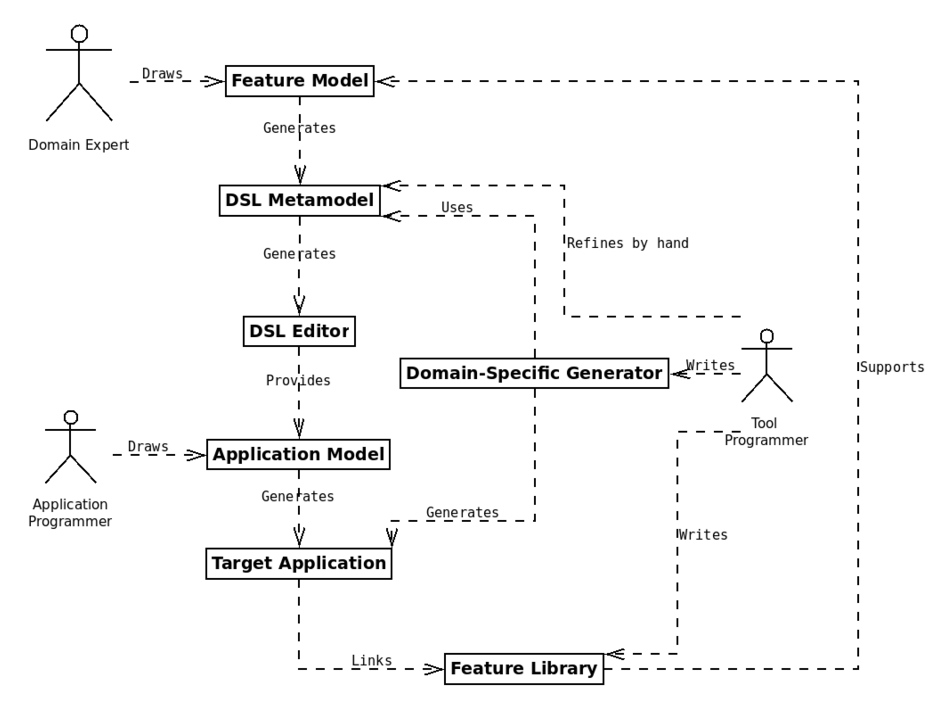
\includegraphics[width=0.76\textwidth]{process.png}
	\caption{Relations between artefacts and roles in proposed approach to domain components reuse.}
	\label{image:process}
\end{figure*}

\section{Proposed approach}
\label{chapter:proposed}
In our approach we will use some ideas of Feature-Oriented Domain Analysis (FODA) method to perform domain analysis and to create feature models. For this we will use visual editor that implements feature diagrams and is easy enough for domain experts. Then, when feature models are ready, each feature is implemented as reusable and configurable component on selected implementation language (C\#, C++, Java and so on) and feature library is formed as a collection of such components. This process requires qualified programmers and requires more effort than to simply create one application, but it allows to reuse features from feature library to create as many applications as needed. Also, this process is scalable, so we may add new features into feature library later, thus allowing to create more complex applications. At this stage of development domain experts shall work with programmers, and they shall use feature diagrams as an input for creation of feature library to simplify matching between features and components in feature library.

Next step is to create domain-specific language that allows to combine and configure features from feature library to implement applications in given domain. This is where our approach differs from common reuse strategies. Naive approach would be to generate an application directly from feature diagram, somehow marking features that shall be included into application, and it actually works fine when domain variability is low~\cite{she2010variability}. But more common is the situation when features themselves have properties that allow to configure them, those properties can have different types. Also, components may be related to each other in different ways, be used in configuration of one another, or some of their properties may be meaningless in absence or presence of other feature. Those rules may be implemented implicitly in application generator and require that programmers will always observe them, but we propose that these rules will be captured explicitly by dedicated domain-specific language. Such language may make models that do not observe those rules syntactically incorrect, and it will greatly reduce the possibility of human error and reduce knowledge required to efficiently use programming system.

By using DSM platforms one can relatively quickly create domain-specific language that will capture domain knowledge, but we already have feature diagram, so we actually can generate the language using it. Generator takes feature diagram as input and produces metamodel of a language. Metamodel is a visual model of a language syntax, that can be opened and edited in yet another visual editor that is part of DSM platform, this editor is called metaeditor. Features from feature diagram become entities in metamodel, this metamodel is then edited to provide shape and a list of properties for each entity. Any vector image can play the role of shape, so the best practise is to select shape that is similar to a feature it depicts. For example, if an application can have buttons, “button” becomes entity in domain-specific language and looks like a button on a diagram. The same happens with properties --- for each feature they are added in metaeditor to corresponding language entity with respect to feature library that actually implements this feature and uses the property to configure it. Properties have name, type and default value. On this step it is also possible to define some constraints on a metamodel that will be checked when model will be edited. If some constraints are violated, user will immediately receive warning, which makes errors in a target application even less likely to occur.

On a next step we use editor generator of the DSM platform to create visual editor for our newly created language. This step if fully automated, and when an editor is generated and loaded into DSM platform, we can use it to create diagrams that specify target applications.

The next thing we need is to generate actual code on target textual language that will call feature library and glue features together. For this we shall return to metamodel level and define generation rules for metamodel. This step is performed only once for a given domain after the feature library and metamodel are finished, and then the same generator is used for each application created by using of the technology. Recommendations for development of domain-specific generator are well-known in DSM literature (for example,~\cite{kelly2008domain}): it is the best to write first application by hand, then draw a model that is supposed to be generated into this application, then find the places in handwritten application that shall be parameterised by information from model and let the generator replace such handwritten parts with data from model. This process is continued until handwritten application becomes a template that is filled by generator with information taken from model. Handwritten application and, consequently, a generator shall extensively use feature library to minimize the amount of code that is generated directly, in ideal case generator shall produce merely a glue code that binds components from feature library together.

After all steps above are finished we have feature library, visual editor for simple domain-specific language that allows to describe how features are combined and configured in a concrete application, and a generator that automatically produces complete application by a model in domain-specific language using feature library as domain-specific runtime~\cite{kelly2008domain}. Now we may create as many applications as we wish by just drawing models and automatically generate complete executable code. Theoretically. Of course, in practise there will always be a need to modify feature diagram, to extend feature library and, consequently, domain-specific language metamodel, modify generator and even to make some changes in generated code, there is no silver bullet. But we believe that our approach can provide better separation of concerns, provides better utilization of domain experts knowledge and expertise among a team. Summary of a process described above and relation between various tools and roles of developers is provided on Fig.~\ref{image:process}.

This approach was implemented in a technology based on QReal DSM platform. QReal became an enabler technology because it provides easy and effective way to create visual editor for domain-specific languages that allows to create fully functional editor in less than an hour. It has visual metaeditor, visual constraints definition tool, visual shape editor and a C++ library that allows to quickly specify generation rules. Feature diagram editor and generator that creates metamodel by feature diagrams were both implemented as plugins to QReal core. Note that feature diagram language is itself domain-specific language for the domain of domain analysis, so it was implemented using QReal metaeditor. The same metaeditor (including shape editor and constraints editor) is then used to tailor the generated metamodel of domain-specific language. Then metaeditor generator is used to generate yet another plugin to QReal that provides visual editor for created language. Then the generator is implemented by hand on C++ with Qt library\footnote{Qt library home page, URL: http://www.qt.io/ (03.04.2016)} using generator creation library included in QReal. Then it is possible to create special distribution of QReal (using Qt Installer framework\footnote{Qt Installer Framework home page, URL: https://wiki.qt.io/Qt-Installer-Framework (03.04.2016)}) that includes only QReal core, editors for feature diagrams (at this point they are needed only as reference) and domain-specific language, generator and feature library, thus forming a complete technology that can be used to generate target applications.

\section{Evaluation}
\label{chapter:evaluation}
For demonstration of the efficiency of proposed above approach there was implemented a model application for remote control of various robot models --- ``Joystick''. The main substantiation for implementing such application is that controlling different robot models requires different control elements. For example, one model can be controlled with only two pads, but another --- with one pad and two buttons. Such application was implemented in C\# for Windows Phone platform. Screenshots of this simple application are presented on Fig.~\ref{image:joystick}. 

\begin{figure*}[t]
	\centering
	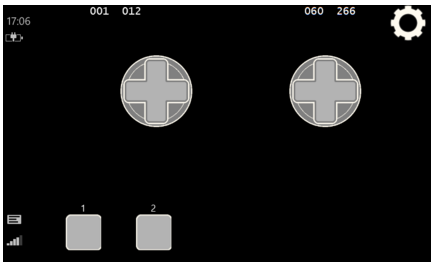
\includegraphics[width=0.35\textwidth]{joystick1.png}
	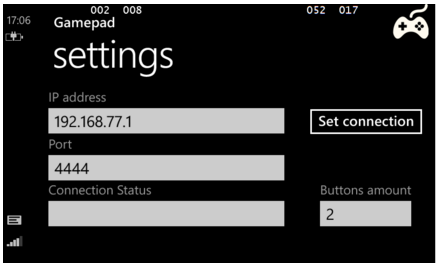
\includegraphics[width=0.35\textwidth]{joystick2.png}
	\caption{Screenshots of ``Joystick'' application.}
	\label{image:joystick}
\end{figure*}


As mentioned above, it was used QReal as DSM tool. A visual language was implemented there for describing feature models. Appropriate feature model for ``Joystick'' application family is proposed on Fig.~\ref{image:joystickFeatureModel}. This feature model presents explicit features, which are labeled as green, and some unite feature groups, which are labeled as blue. Type of arrow shows which feature is compulsory (shown as solid line with arrow on the end), which compulsory but there is some alternative between them (shown as dash line with an arrow on the end), and optional features, which may be implemented but not compulsory (shown as dash line with a circle on the end).

\begin{figure}[H]
	\centering
	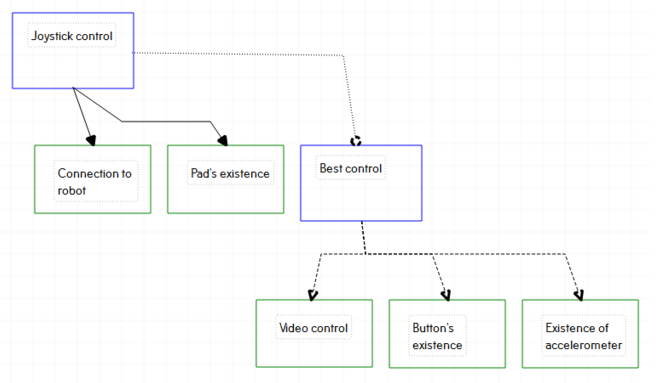
\includegraphics[width=0.5\textwidth]{joystickFeatureModel.png}
	\caption{Feature model for ``Joystick'' application family.}
	\label{image:joystickFeatureModel}
\end{figure}

Based on this feature model a metamodel for future visual language was generated, which is required for building different models for different configurations. Generated metamodel is presented on Fig.~\ref{image:joystickMetamodel}. As it can be seen, metamodel is very simple. At this stage we can propose that entities, such as ``buttons'' and ``pads'', may have a property ``Quantity''. In addition, we can specify images for these entities, which will be shown in visual language. 

\begin{figure}[H]
	\centering
	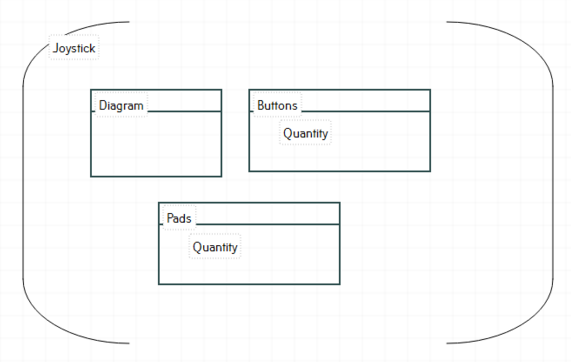
\includegraphics[width=0.5\textwidth]{joystickMetamodel.png}
	\caption{Metamodel of visual language for ``Joystick'' application family.}
	\label{image:joystickMetamodel}
\end{figure}

Then with the aid of QReal tool a visual language was generated. Example of generated visual language is demonstrated on Fig.~\ref{image:joystickDsl}. It can be seen that in visual language editor can be specified property ``Quantity'', explicitly noting the concrete number of pads. 


\begin{figure}[H]
	\centering
	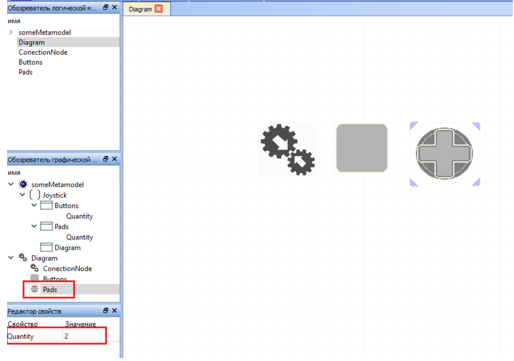
\includegraphics[width=0.5\textwidth]{joystickDsl.png}
	\caption{Visual language for ``Joystick'' application family.}
	\label{image:joystickDsl}
\end{figure}

As can be seen, example is quite simple for demonstrating extensive possibilities of the approach proposed above. At present there is no rigorous evaluation of the proposed process. Also, cohesive and consistent technology for creating application family based on domain analysis is not implemented yet, here we have described a concept-proof prototype. Therefore, this work requires more detailed explorations.

\section{Conclusion}
\label{chapter:conclusion}
The problem of not using domain analysis result for further generation of some entities for software development process was stated. There were considered some formal domain analysis approaches and we concluded that creation of feature diagrams is the most elegant decision for domain analysis that can be conducted by domain expert, i.e. non-programmer, maybe in collaboration with system analysts. Moreover, there was discussed one of the possible solutions, which is presented by Estublier, we specify some problems of such method. We suggested our own approach for creation of application family in one domain based on domain analysis. Thus, some target applications can be implemented even by non-programmers using domain-specific language with configurating features from library. Also, there was some evaluation of this approach, where we pointed out that this example remains many questions because of its simplicity.


\bibliographystyle{utf8gost705u}
\bibliography{bibliography}

\end{document}